%General
\documentclass{article}
\usepackage[utf8]{inputenc}
\usepackage{fullpage}

%Symbols
\usepackage{commath}
\usepackage{amsmath}
\usepackage{amssymb}
\usepackage{tikz}
\usetikzlibrary{arrows,automata}

%Formatting
\usepackage{enumerate}
\usepackage{bussproofs}
\usepackage{hyperref}
\usepackage{amsthm}
\usepackage{alltt}
\newtheorem{theorem}{Theorem}[section]
\newtheorem{definition}[theorem]{Definition}
\newtheorem{example}[theorem]{Example}
\hypersetup{colorlinks=true}
\hypersetup{colorlinks=true}
\usepackage{graphicx}
\graphicspath{ {img/} }
\usepackage{caption}

\title{$\epsilon$-NFA and RE}
\date{\today}
\author{Rikard Hjort}

\begin{document}
\maketitle

\section*{Problem 1}

We denote the given $\epsilon$-NFA $N = (Q_E, \Sigma, \delta_E, q_0, F_E)$ where these symbols have their usual meaning. In this case $Q_E = \set{q_0, q_1, q_2, q_3, q_4, q_5}$, $\Sigma = \set{0,1}$ and $F = \set{q_5}$. We create the DFA $D$, which, as any DFA, is the 5-tuple

$$D = (Q_D, \Sigma, \delta_D, q_D, F_D)$$

where $Q_D$ is the $\epsilon$-closure of every set in the power set of $Q_E$, $q_D$ is the $\epsilon$-closure of $\set{q_0}$, $F_D$ is the set of all sets in $Q_D$ in which at least one state is in $F_E$, and $\delta_D$ is the transition function we seek to construct. 

We will ommit from our description of $D$ any state in $Q_D$ which is not reachable, to avoid enumrating and describing superfluous states. We will also refrain from defining $F_D$ until we have constructed the transition function, for the same reason. When constructing $\delta_D$ we will find out which states are reachable. However, we can note right away that $q_D = ECLOSE(\set{q_0}) = \set{q_0, q_1, q_3, q_5}$

We construct the transition function iteratively by going over every state in $q_D$ and take the union of the resulting state for each input symbol. More formally, we will start by finding $\Delta (q_D, a) = \bigcup_{s \in q_D}\delta_E(s, a)$. We then caculate the $\epsilon$-closure of $\Delta(q_D, a)$ to obtain a new set of states in $Q_E$. We add this set as a state in $D$. For each such new state, we repeat the above procedure.

\begin{align*}
    ECLOSE(\Delta(q_D,0)) &=ECLOSE(\Delta(\set{q_0, q_1,q_3,q_5}, 0)) = ECLOSE(\set{q_1,q_3,q_5}) = \set{q_1, q_3, q_5} \\
    ECLOSE(\Delta(q_D,1)) &=ECLOSE(\Delta(\set{q_0, q_1,q_3,q_5}, 1)) = ECLOSE(\set{q_0, q_1, q_3, q_4, q_5}) = \set{q_0,q_1, q_3,q_4, q_5}
\end{align*}

We repeat the procedure for $\set{q_1,q_3,q_5}$ and $\set{q_0, q_1, q_3, q_4, q_5}$, and then for the results of these states, and so forth.

Finally we find that $D$ is described by the following transition table.

\begin{align*}
    \begin{array}{r||l| l}
         &0 & 1 \\ \hline
        \to ^*\set{q_0,q_1,q_3,q_5} & \set{q_1, q_3, q_5} & \set{q_0, q_1,q_2,q_3,q_4,q_5} \\
        ^*\set{q_1, q_3, q_5} & \set{q_3,q_5} & \set{q_1, q_3, q_4, q_5}\\
        ^*\set{q_0, q_1,q_2,q_3,q_4,q_5} & \set{q_1, q_3, q_5} & \set{q_0, q_1,q_2,q_3,q_4,q_5} \\
        ^*\set{q_3,q_5} & \set{q_5} & \set{q_3,q_5}\\
        ^*\set{q_1, q_3, q_4, q_5} & \set{q_3,q_5} & \set{q_1,q_3,q_4, q_5}\\
        ^*\set{q_5} & - & -
    \end{array}
\end{align*}

\newpage
\section*{Problem 2}

\begin{figure}[htpb]
    \centering
    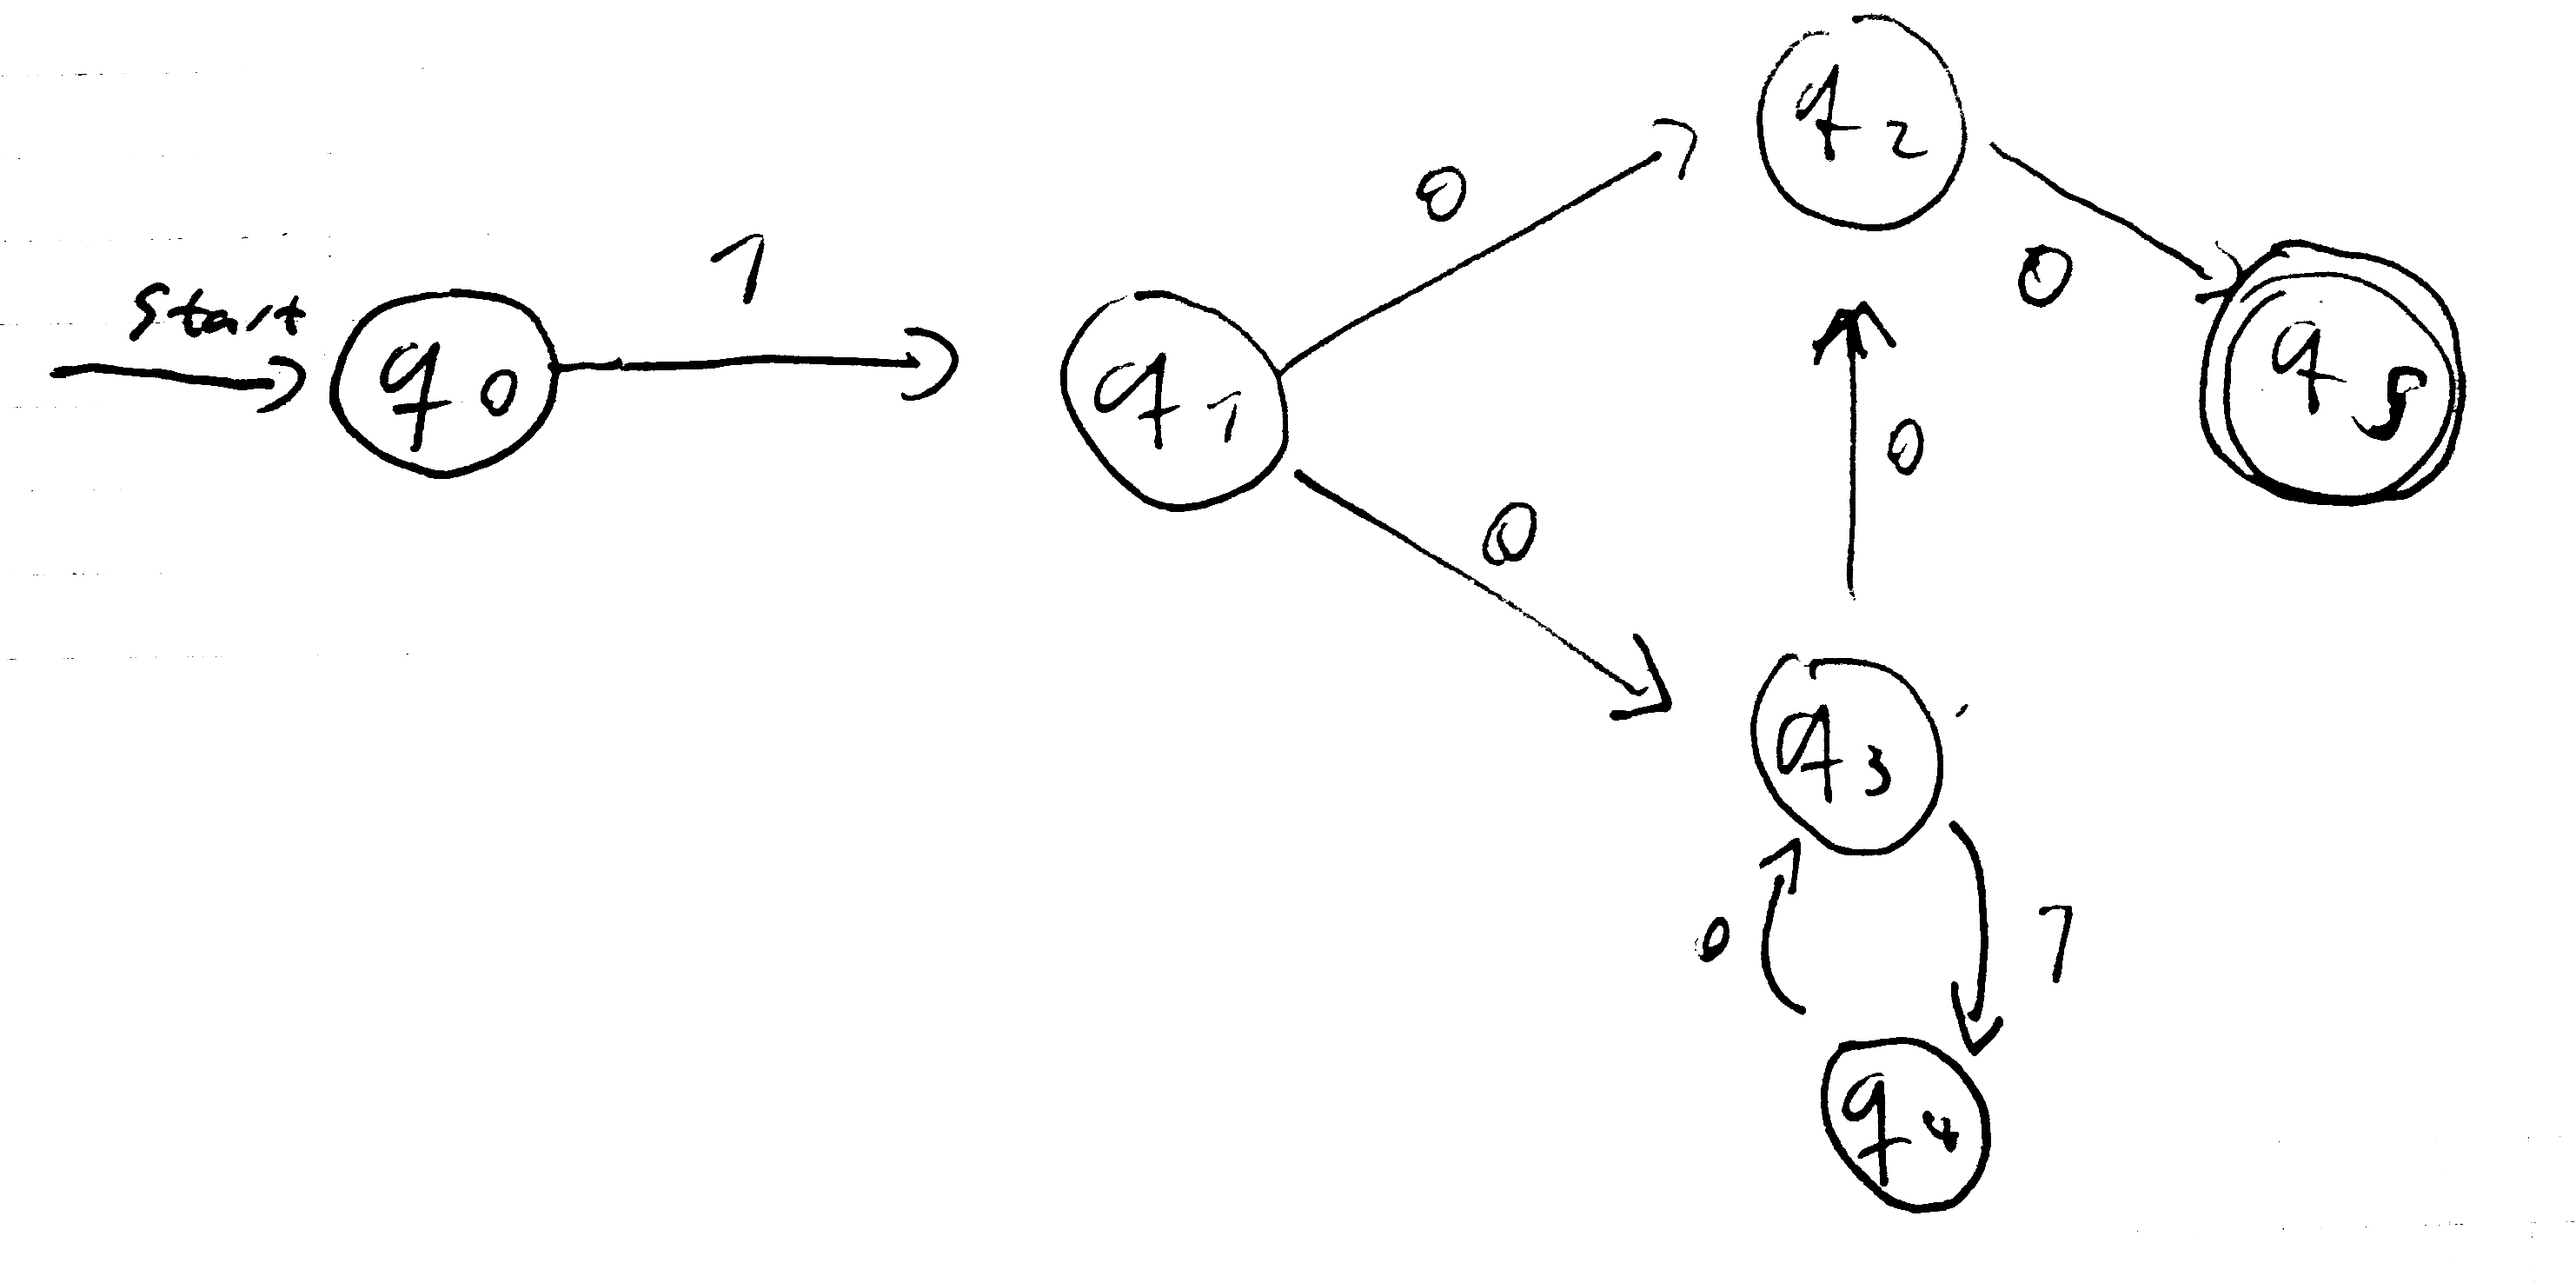
\includegraphics[width=0.8\linewidth]{nfa}
    \caption{An NFA accepting the same language as the regular expression $1(0 + 0(10)^*0)0$.}
\end{figure}

\newpage
\section*{Problem 3}

It helps me to first create an $\epsilon$-NFA that accepts this language. This is easy. We simply create an automaton that has two branches: one that remembers if we have encountered an even number of 1's, and one if we've encountered a multiple of 3 symbols. This automaton can be seen in figure \ref{fig:epsnfa}.

\begin{figure}[htpb]
    \centering
    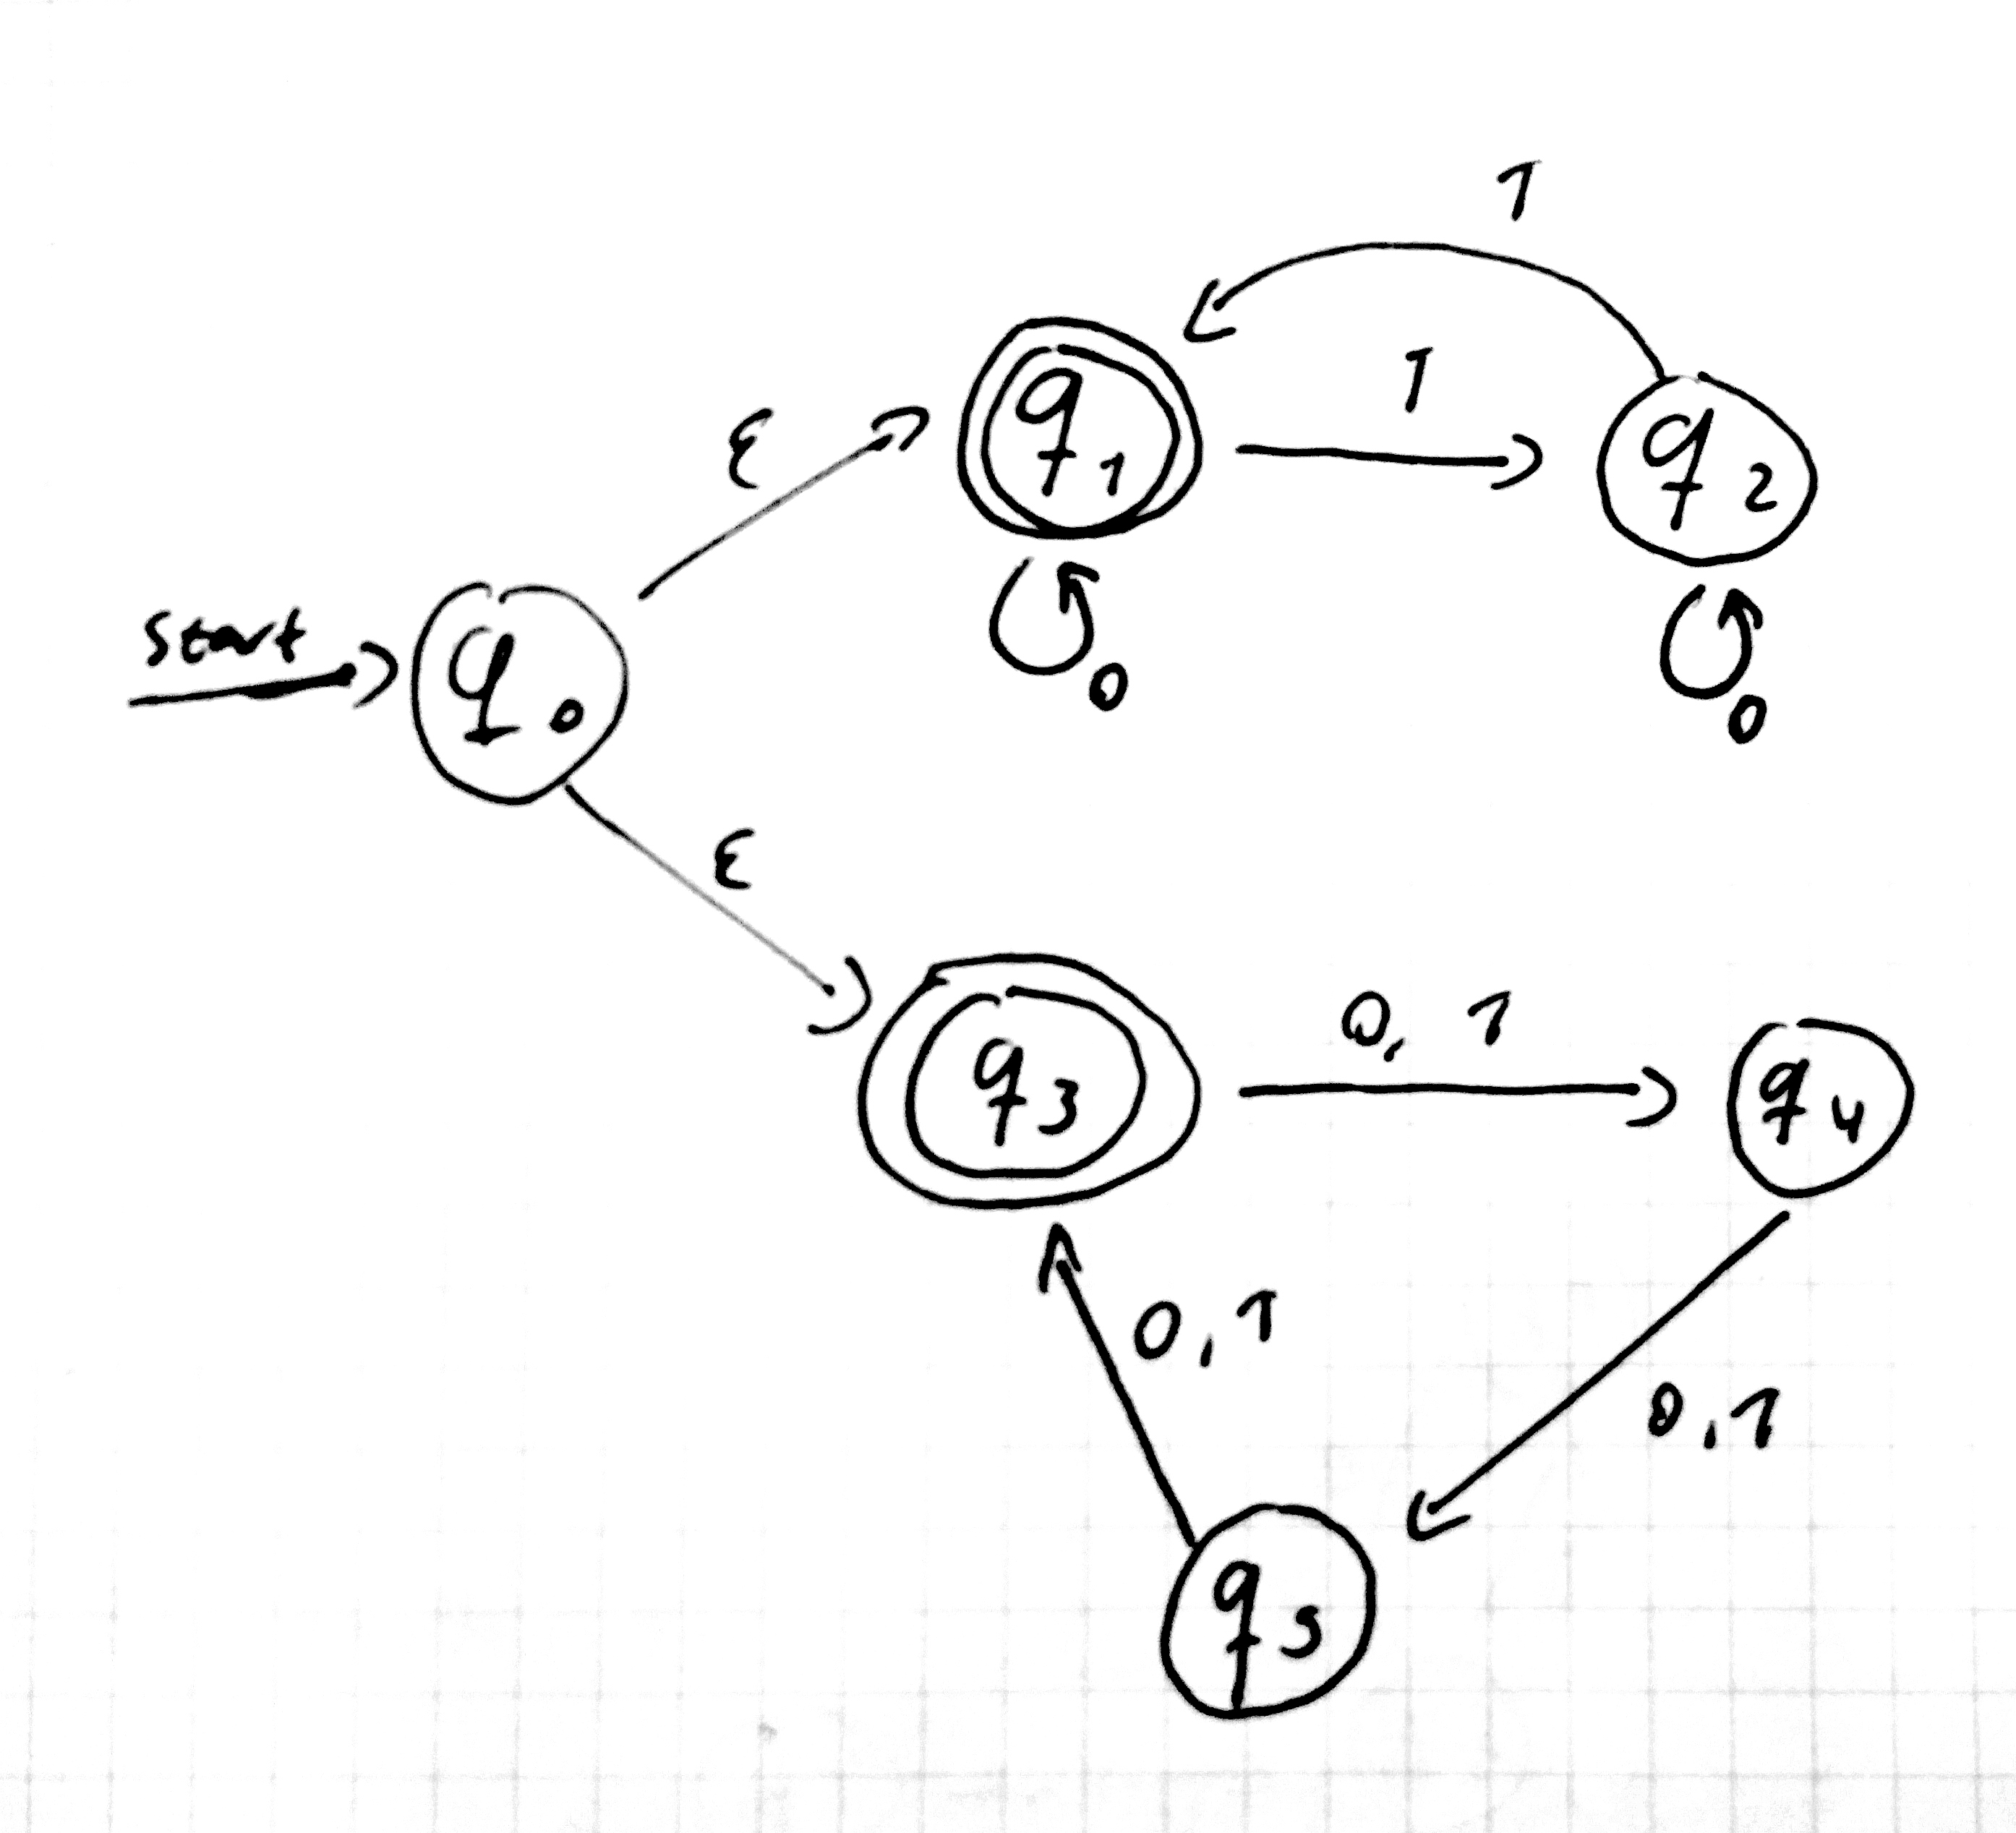
\includegraphics[width=0.8\linewidth]{epsnfa}
    \caption{An $\epsilon$-NFA accepting the language of words containing an even number of 1's or a multiple of 3 symbols.}
    \label{fig:epsnfa}
\end{figure}

This automaton can now be reduced by simply eliminating states. First, we eliminate $q_2$, resulting in a loop from $q_1$ to itself with the label $0+10^*1$, since we can either go to $q_1$ by reading 0, or byr reading a 1, followed by any number of 0's, and then reading 1 again.

We then remove state $q_4$ by adding an arc from $q_3$ to $q_5$ with the label $(0+1)(0+1)$ and removing all arcs to and from $q_4$. We eliminate $q_5$ by creating a loop from $q_3$ to itself with the label $(0+1)(0+1)(0+1)$.

The result of these two reductions can be seen in figure \ref{fig:epsnfa-eliminated}.

\begin{figure}[htpb]
    \centering
    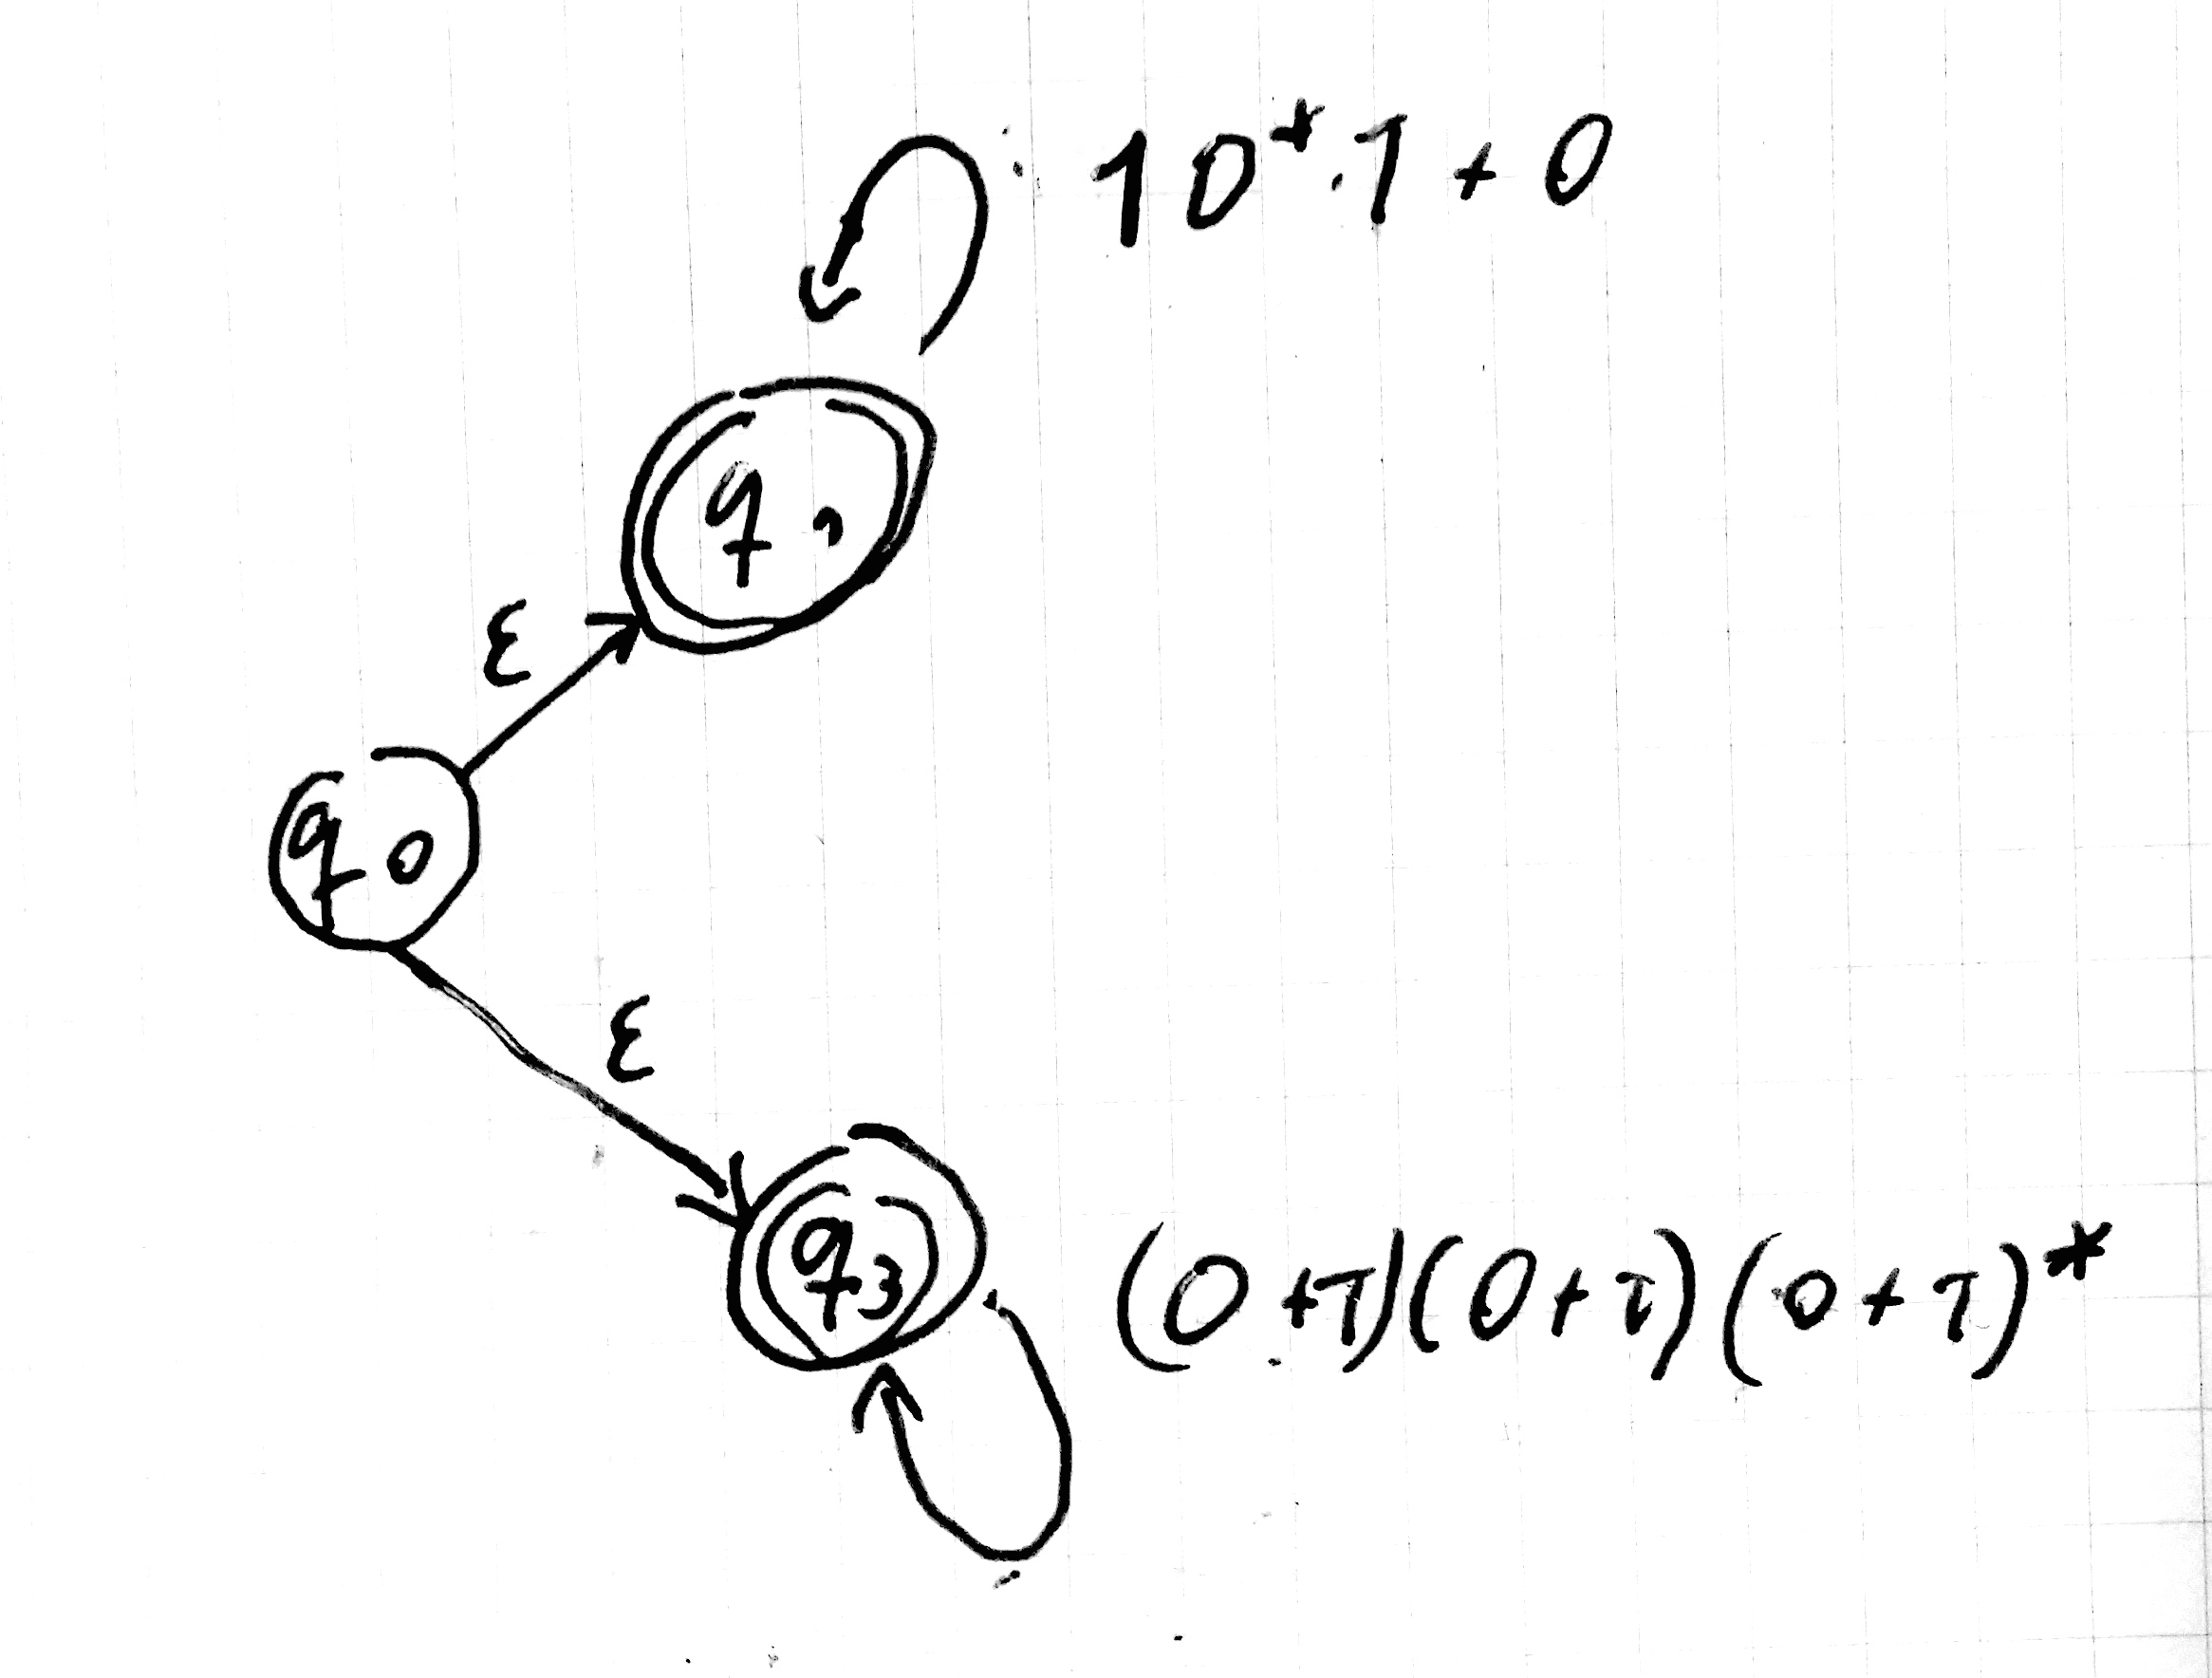
\includegraphics[width=0.8\linewidth]{epsnfa-eliminated}
    \caption{The NFA in figure \ref{fig:epsnfa} after eliminating states $q_2,q_4,q_5$}
    \label{fig:epsnfa-eliminated}
\end{figure}

When we eliminate $q_1$, we are left with the expression $((0+1)(0+1)(0+1))^*$, and when we eliminate $q_3$ we are left with the expression $(10^*1+0)^*$. Thus, the entire regular expression requested in the problem is $(10^*1+0)^* + ((0+1)(0+1)(0+1))^*$

\newpage
\section*{Problem 4}

\begin{enumerate}[(a)]
    \item 
        Initially, the automaton looks like figure \ref{fig:4_1}. We begin by eliminating state $q_1$. We do this by going to the transition table and for each state, identifying any transition from that state to $q_1$. We replace this transition with a regular expression $RS*T$, where $R$ is the symbol that causes a transition to $q_1$, $S$ is a symbol that loops back to $q_1$, and $T$ is a symbol which transitions from $q_1$ to another state. 

\begin{figure}[htpb]
    \centering
    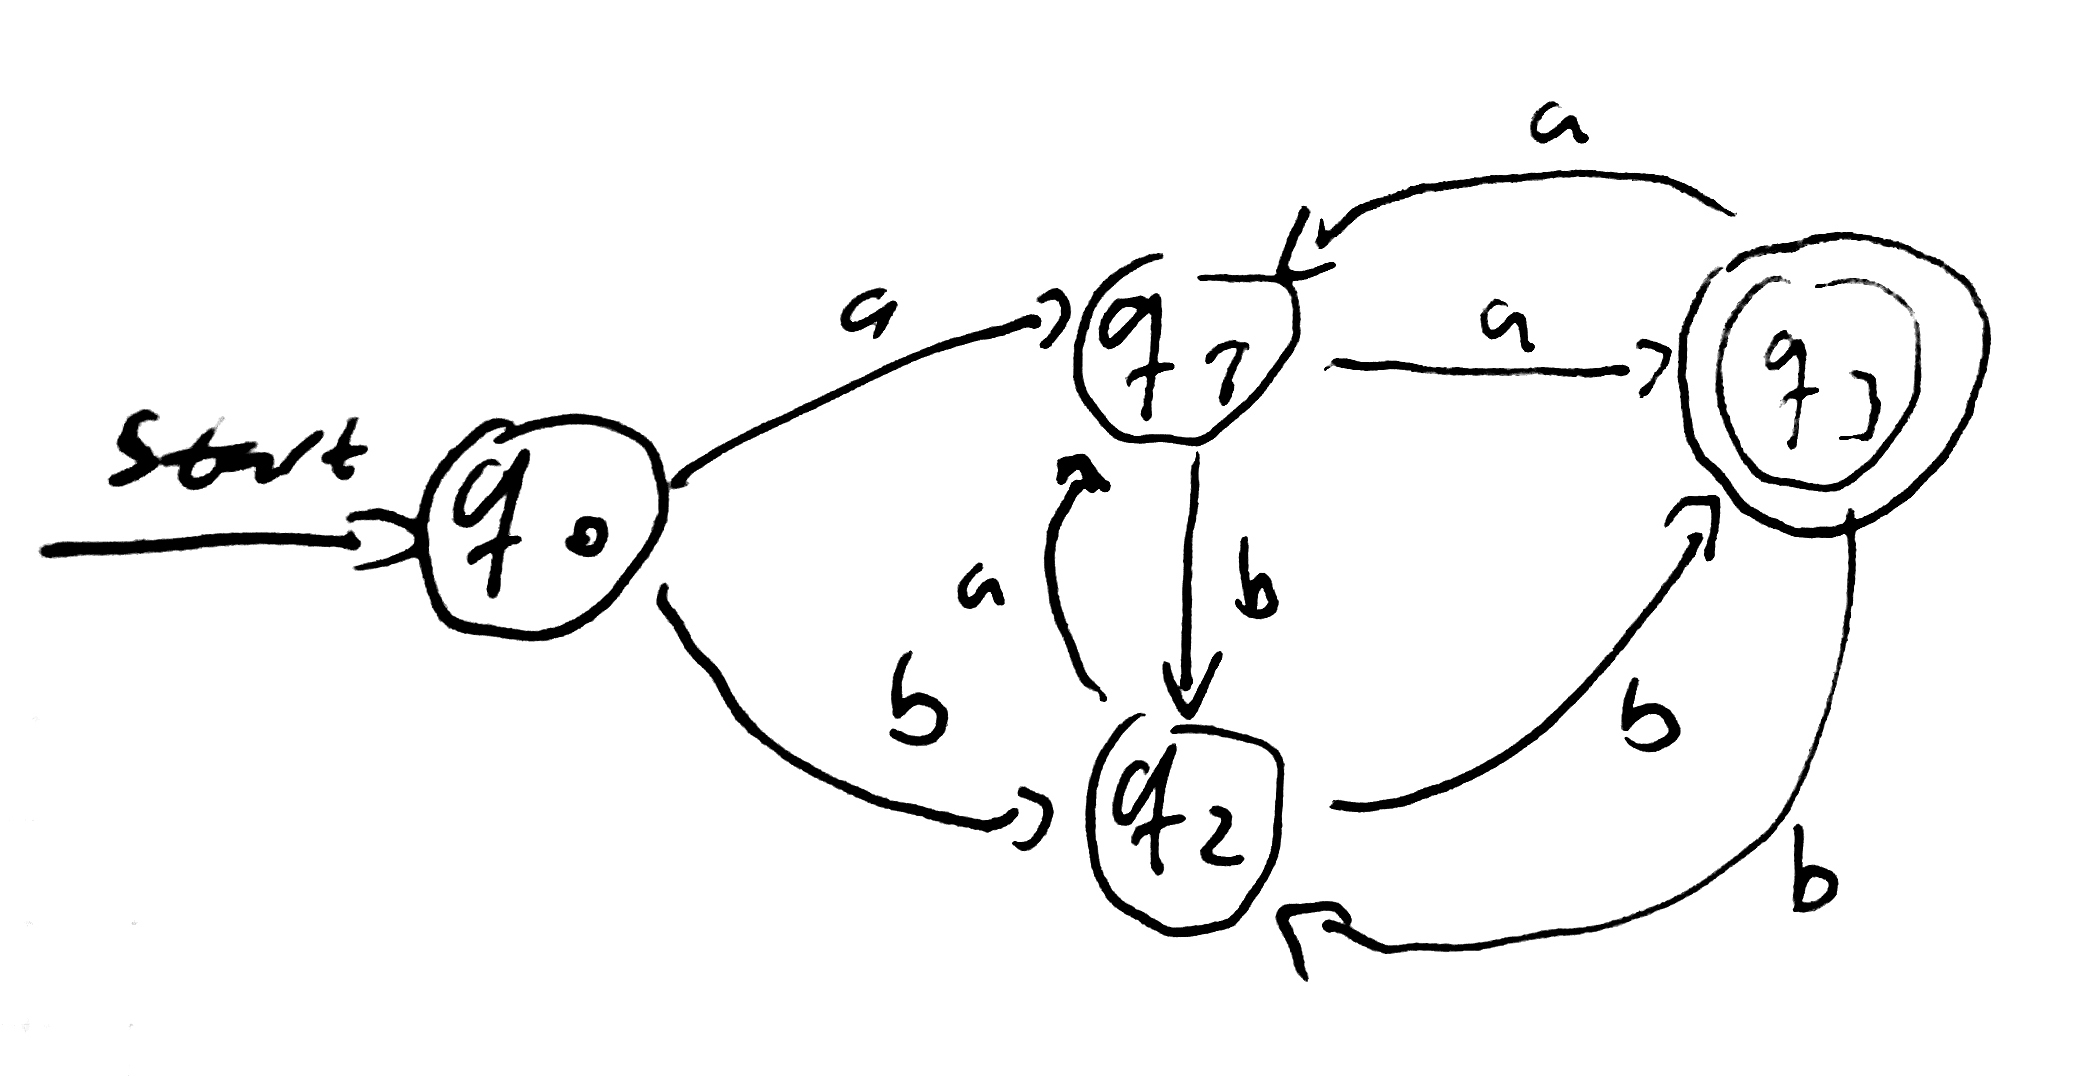
\includegraphics[width=0.8\linewidth]{week3_4_1}
    \caption{The original automaton.}
    \label{fig:4_1}
\end{figure}

        We do not need to consider the expression $S$ in this first step, since there is no loop from $q_1$ to itself. After eliminiating $q_1$, there is a new arc from $q_0$ to $q_3$ labeled $\mathbf{aa}$, from $q_0$ to $q_2$ labeled $\mathbf{ab}$, from $q_2$ to itself labeled $\mathbf{ab}$, from $q_2$ to $q_3$ labeled $\mathbf{aa}$, from $q_3$ to itself labeled $\mathbf{aa}$ and from $q_3$ to $q_2$ labeled $\mathbf{ab}$. Combining these new arcs with all existing ones between the remaining states, we get the automaton in figure \ref{fig:4_2}.

\begin{figure}[htpb]
    \centering
    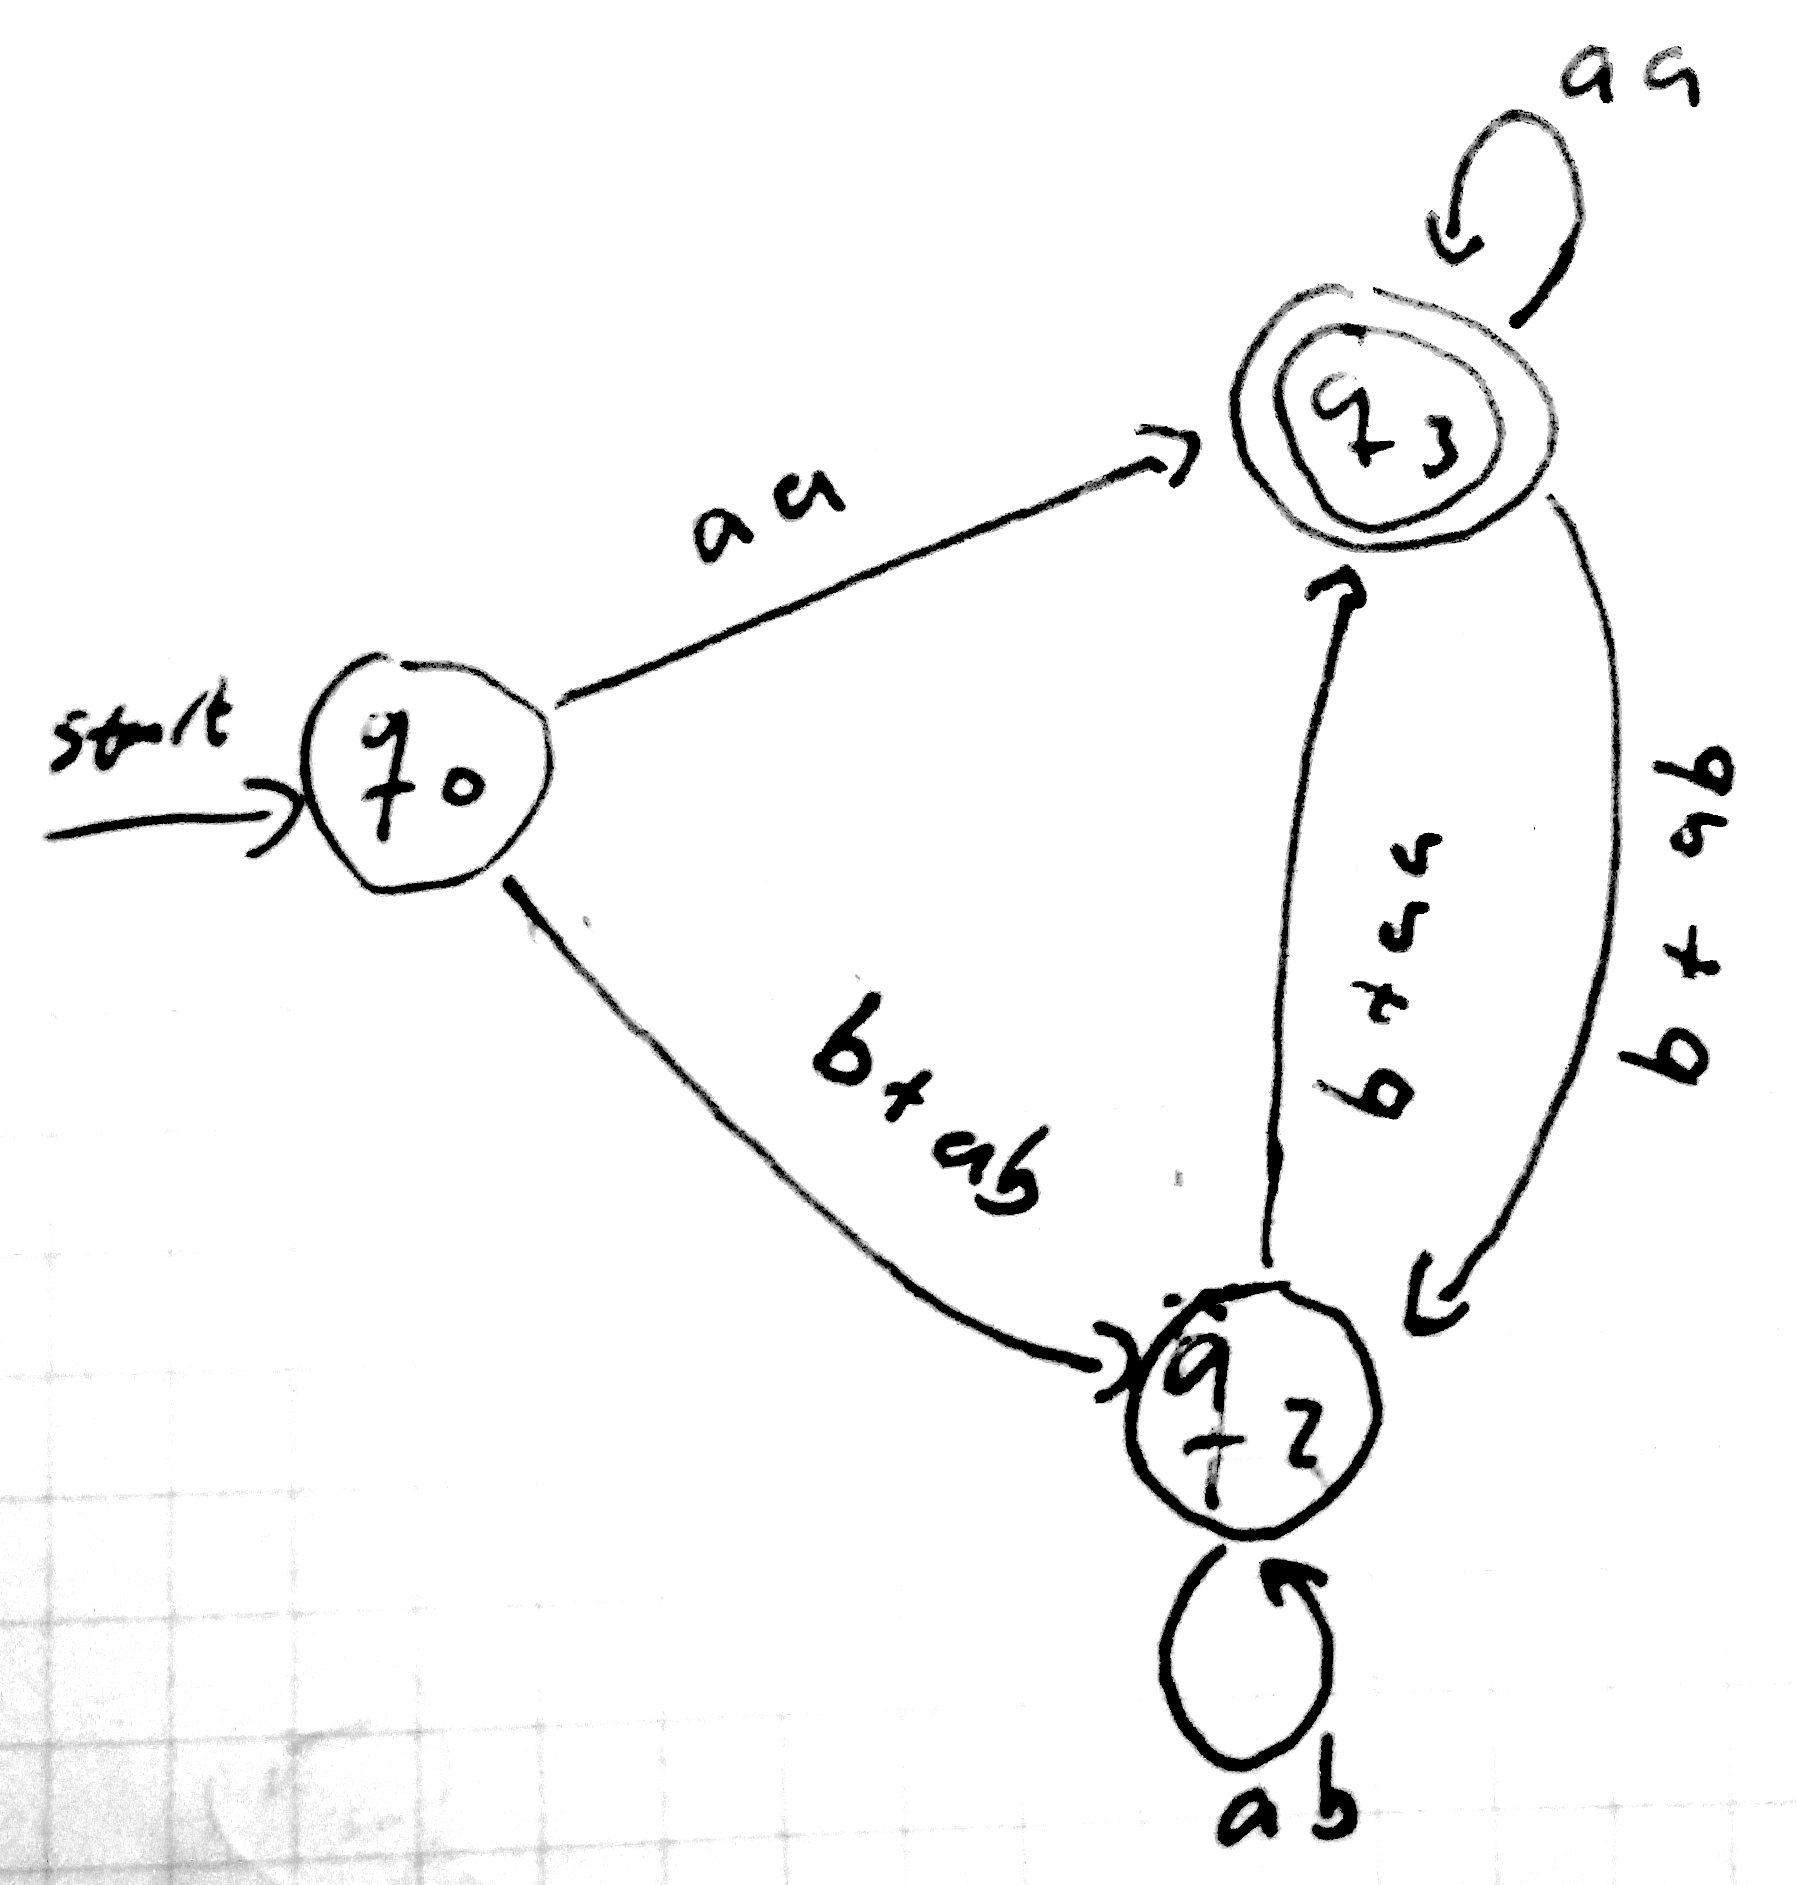
\includegraphics[width=0.6\linewidth]{week3_4_2}
    \caption{The automaton with state $q_1$ eliminated.}
    \label{fig:4_2}
\end{figure}

We now eliminate state $q_2$ and get the automaton in figure \ref{fig:4_3}. 

\begin{figure}[htpb]
    \centering
    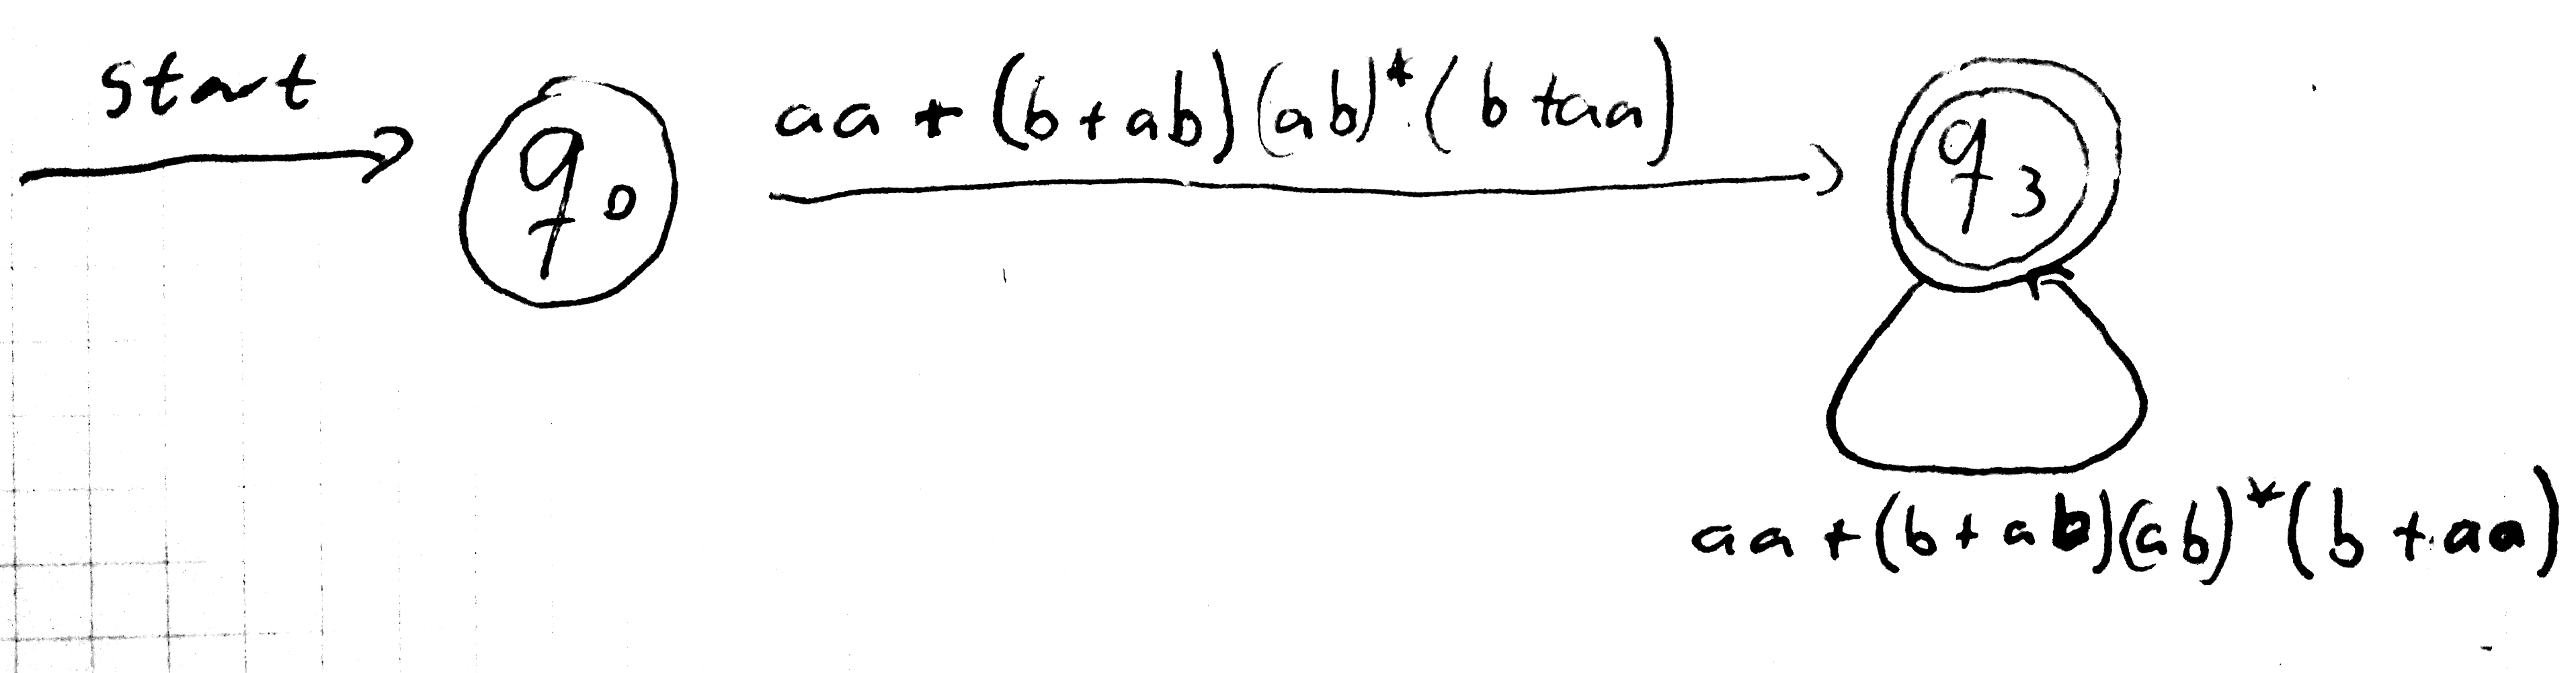
\includegraphics[width=0.8\linewidth]{week3_4_3}
    \caption{The automaton with states $q_1$ and $q_2$ eliminated.}
    \label{fig:4_3}
\end{figure}

From this automaton we can construct the final regular expression. We begin by noting that the expressions on both arcs are identical. We will call this expression $R$. Now, to transition to the final state, we must go along the arc from the initial state to the final state, and then remain there by only reading strings generated by $R$. We can conclude that the automaton accepts the language

$$RR^* = R^+= \mathbf{(aa+(b+ab)(ab)^*(b+aa))^+}$$

This regular expression generates the same language as the automaton.

\item
    We state the transition from every state $q_i$ to the accepting state $q_3$ with equation $E_i$.

    \begin{align*}
        E_0 &= \mathbf{a}E_1 + \mathbf{b}E_2 \\
        E_1 &= \mathbf{a}E_3 + \mathbf{b}E_2 \\
        E_2 &= \mathbf{a}E_1 + \mathbf{b}E_3 \\
        E_3 &= \epsilon + \mathbf{a}E_1 + \mathbf{b}E_2
    \end{align*}

    We procede to eliminate $E_1$, simplifying with help of the rules of associativity of concatenation for languages along the way.

    \begin{equation*}
    \centering
    \begin{array}{l l l}
        E_0 &= \mathbf{aa}E_3 + \mathbf{ab}E_2 + \mathbf{b}E_2 &= \mathbf{aa}E_3 + (\mathbf{a} + \epsilon)\mathbf{b}E_2  \\
        E_2 &= \mathbf{aa}E_3 + \mathbf{ab}E_2 + \mathbf{b}E_3 &= (\mathbf{aa}+\mathbf{b})E_3 + \mathbf{ab}E_2\\
        E_3 &= \epsilon + \mathbf{aa}E_3 + \mathbf{ab}E_2 + \mathbf{b}E_2 &= \epsilon + \mathbf{aa}E_3 + (\mathbf{a}+\epsilon)\mathbf{b}E_2
    \end{array}
    \end{equation*}
    
    We repeat the procedure and eliminate $q_2$, using Arden's lemma to get rid of recursive definitions of expressions.

    \begin{equation*}
    \centering
    \begin{array}{l l l}
        E_0 &= \mathbf{aa}E_3 + (\mathbf{a}+\epsilon)\mathbf{b}(\mathbf{ab})^*(\mathbf{aa}+\mathbf{b})E_3 &= (\mathbf{aa} + (\mathbf{a}+\epsilon)\mathbf{b}(\mathbf{ab})*(\mathbf{aa}+\mathbf{b}))E_3 \\
        E_3 &= \epsilon + \mathbf{aa}E_3+ (\mathbf{a}+\epsilon)\mathbf{b}(\mathbf{ab})^*(\mathbf{aa}+\mathbf{b})E_3 &= \epsilon + (\mathbf{aa} + (\mathbf{a}+\epsilon)\mathbf{b}(\mathbf{ab})^*(\mathbf{aa}+\mathbf{b}))E_3
    \end{array}
    \end{equation*}

    We then eliminate $q_3$.

    \begin{equation*}
    \centering
    \begin{array}{l l l}
        E_0 &= (\mathbf{aa} + (\mathbf{a}+\epsilon)\mathbf{b}(\mathbf{ab})^*(\mathbf{aa}+\mathbf{b}))(\mathbf{aa} + (\mathbf{a}+\epsilon)\mathbf{b}(\mathbf{ab})^*(\mathbf{aa}+\mathbf{b}))^* &= (\mathbf{aa} + (\mathbf{a}+\epsilon)\mathbf{b}(\mathbf{ab})^*(\mathbf{aa}+\mathbf{b}))^+\\
    \end{array}
    \end{equation*}

    Finally, expanding the concatenation $\mathbf{(a+\epsilon)b}$ using the distributive law of languages, we get

    $$E_0 = \mathbf{(aa+(b+ab)(ab)^*(b+aa))^+}$$

    This is a regular expression accpeting the same language as the automaton.

\end{enumerate}
\end{document}
